% LyX 2.0.5.1 created this file.  For more info, see http://www.lyx.org/.
%% Do not edit unless you really know what you are doing.
\documentclass[12pt]{report}
\usepackage{mathptmx}
\renewcommand{\familydefault}{\rmdefault}
\usepackage[T1]{fontenc}
\usepackage[latin9]{inputenc}
\usepackage[a4paper]{geometry}
\geometry{verbose,tmargin=2cm,bmargin=2cm,lmargin=2cm,rmargin=2cm,headheight=1cm,headsep=1cm,footskip=1cm}
\setcounter{secnumdepth}{2} % Changed from 3 to 2. 0-chapter 1-section 2-subsection 
\setcounter{tocdepth}{2} % Changed from 3 to 2. 0-chapter 1-section 2-subsection 
\setlength{\parskip}{\medskipamount}
\setlength{\parindent}{0pt}
\usepackage{verbatim}
\usepackage{pdfpages}
\usepackage{graphicx}
\usepackage{subfigure}
\usepackage{setspace}
\usepackage[numbers]{natbib}
\usepackage{nomencl}
% the following is useful when we have the old nomencl.sty package
\providecommand{\printnomenclature}{\printglossary}
\providecommand{\makenomenclature}{\makeglossary}
\makenomenclature
\doublespacing

\makeatletter

%%%%%%%%%%%%%%%%%%%%%%%%%%%%%% LyX specific LaTeX commands.
\providecommand{\LyX}{L\kern-.1667em\lower.25em\hbox{Y}\kern-.125emX\@}
%% Because html converters don't know tabularnewline
\providecommand{\tabularnewline}{\\}
%% A simple dot to overcome graphicx limitations
\newcommand{\lyxdot}{.}


%%%%%%%%%%%%%%%%%%%%%%%%%%%%%% User specified LaTeX commands.
\usepackage{tauthesis}
\usepackage[font={small,bf}, labelfont={small,bf}, margin=1cm]{caption}
\usepackage{titlesec}
\newcommand{\hsp}{\hspace{20pt}}
\titleformat{\chapter}[hang]{\Huge\bfseries}{\thechapter\hsp}{0pt}{\Huge\bfseries}

\newcommand{\nb}{NetBatch}
\newcommand{\fif}{First-Fit}
\newcommand{\bef}{Best-Fit}
\newcommand{\wof}{Worse-Fit}
\newcommand{\mif}{Mix-Fit}
\newcommand{\maj}{Max-Jobs}
\newcommand{\wfc}{Worse-Fit-Cores}
\newcommand{\wfm}{Worse-Fit-Memory}
\newcommand{\bfc}{Best-Fit-Cores}
\newcommand{\bfm}{Best-Fit-Memory}


\Title{\textbf{Heuristics for Resource Matching\\in Intel's Compute Farm}}
\Author{Ohad Shai}
\Year{August 2014}
\Supervisor{Prof. Dror G. Feitelson}
\Department{Blavatnik School of Computer Science}
\Degree{Master of Science}
% \Degree{Doctor of Philosophy}

\makeatother

\begin{document}
\begin{comment}
This is Micheal JasonSmith's uocthesis example ported to \LyX{} by
Etienne Lalibert� (etiennlaliberte@gmail.com).

Alex Liberzon (alex.liberzon@gmail.com) modified it to the Tel Aviv
University format, with the logo of the Faculty of Engineering. Change
the file taulogo.png to get the logo of your department.

Go to \textsf{Document > Settings > \LaTeX{} preamble} to modify the
\textsf{Title, Author, Year, Supervisor, Department} fields.

Default processor is now DVIPDFM - but if you can choose something
else, try PDFLATEX and XELATEX - sometimes these are a bit faster. 
\end{comment}


\prelimpages

\titlepage

\acknowledgments{
I would like to express my gratitude to those who without them this research would not have been completed.

I would like to thank my advisor Prof. Dror Feitelson for his guidance of my first steps
in the world of job scheduling. His vast experience in that field was of a great
benefit for me, His patience and the atmosphere of the work are very much appreciated.

I would like to thank Dr. Edi Shmueli for his part in the research. Without
his motivation, partnership and guidance I cannot imagine the research.

In addition, I would like to thank my managers at Intel, Nir Antebi and Moshe Sananes who gave me the
appropriate ground and the required assistance for the study at Intel.

I would like to thank Prof. Sivan Toledo for the escort of the research in Tel Aviv University allowing 
that non-standard setup.

Last, I would like to thank my family. My parents Anat and Eran for their encouragement and support throughout my studies. 
My loved wife Yael and my children Roni and Tomer for giving me that opportunity and their encouragement throughout my studies.

}

\begin{comment}
Split the thesis into separate chapters. Use \textbackslash{}include
mode to include the separate files.

Use \LyX{} Table of Contents, List of Figures, List of Tables and
Nomenclature automatics to include them in the thesis. Double - click
on each item to change the default level of contents, move the chapters
up/down and so on.
\end{comment}

\cleardoublepage
\setcounter{page}{1} % Start preliminary pages numbering (roman numerals).
%% LyX 2.0.5.1 created this file.  For more info, see http://www.lyx.org/.
%% Do not edit unless you really know what you are doing.

\chapter*{Abstract}

In this paper we investigate the issue of resource matching between jobs and machines in Intel's compute farm. We show that common heuristics such as Best-Fit and Worse-Fit may fail to properly utilize the available resources when applied to either cores or memory in isolation. In an attempt to overcome the problem we propose Mix-Fit, a heuristic which attempts to balance usage between resources. While this indeed usually improves upon the single-resource heuristics, it too fails to be optimal in all cases. As a solution we default to Max-Jobs, a meta-heuristic that employs all the other heuristics as sub-routines, and selects the one which matches the highest number of jobs. Extensive simulations that are based on real workload traces from four different Intel sites demonstrate that Max-Jobs is indeed the most robust heuristic for diverse workloads and system configurations, and provides up to 22% reduction in the average wait time of jobs.  


    

\tableofcontents{}

\listoffigures

\listoftables

\printnomenclature{}

\textpages


%main section

\begin{spacing}{1.8}


\chapter{Introduction}
%=====================

Intel owns an Internet-scale distributed compute farm that is used for
running its massive chip-simulation workloads
\cite[p.\ 78]{bentley01,evans03:book}.
The farm is composed of tens of thousands of servers that are located
in multiple data centers that are geographically spread around the
globe.
It is capable of running hundreds of thousands of simulation jobs and
tests simultaneously, and handles a rate of thousands of newly
incoming jobs every second.

This huge compute capacity is managed by an in-house developed
highly-scalable two-tier resource management and scheduling system
called \nb.
At the lower level \nb\ groups the servers into autonomous clusters
that are referred to in \nb\ terminology as Physical Pools.
Each such pool contains up to thousands of servers and is managed by a
single \nb\ entity that is called the Physical Pool Manager or PPM.
The role of the PPM is to accept jobs from the upper level, and to
schedule them on underlying servers efficiently and with minimal
waste.

At the upper level \nb\ deploys a second set of pools that are called
Virtual Pools.
Just like in the lower level, each virtual pool is managed by a single
\nb\ component that is called the Virtual Pool Manager or VPM.
The role of the VPMs is to cooperatively accept jobs from the users
and distribute them to the different PPMs in order to spread the load
across the farm.
Together, these two layers, VPMs at the top and PPMs at the
bottom, strive to utilize every compute resource across the farm.
This work focuses on the work done at the PPM level.

A basic requirement in \nb\ is the enforcement of fair-share
scheduling among the various projects and business units within Intel
that share the farm.
Fair-share begins at the planning phase where different projects
purchase different amounts of servers to be used for their jobs.
These purchases eventually reflect their share of the combined
resources.
Once the shares are calculated, they are propagated to the PPMs where
they are physically enforced. The calculation and propagation
mechanisms are beyond our scope.

To enforce fair-share the PPM constantly monitors which jobs from
which projects are currently running and the amount of resources they
use.
The PPM then selects from its wait queue the first job from the most
eligible project (the project whose ratio of currently used resources
to its share of the resources is the smallest) and tries to match a
machine to that job.
If the matching succeeds, the job is scheduled for execution on that
machine.
Otherwise, a reservation is made for the job, and the process is
repeated while making sure not to violate previously made
reservations.
Such reservations enable jobs from projects that are lagging behind to
obtain the required resources as soon as possible.

Matching machines to jobs is done using any of a set of heuristics.
For example, one may sort the list of candidate machines according to
some pre-defined criteria --- e.g.\ increasing number of free cores or
decreasing amount of free memory --- and then traverse the sorted list
and select the first machine on which the job fits.
This leads to variants of \bef\ and \wof\ schemes.
Good sorting criteria reduce fragmentation thus allowing more jobs to be
executed, and are critical for the overall utilization of the pool.
Alternatively one may opt to reduce overhead and use a
\fif\ heuristic.

The sorting criteria are programmable configuration parameters in \nb.
This allows one to implement various matching heuristics and apply
them on different resources to best suit the workload characteristics
and needs.
\nb\ also allows individual jobs to specify different heuristics,
while the pool administrator can set a default policy to be used for
all jobs.

In this work we argue that no heuristic applied to a
single resource in isolation can yield optimal performance under all
scenarios and cases.
To demonstrate our point we use both simple test cases and workload
traces that were collected at four large Intel sites.
Using the traces, we simulate the PPM behavior when applying the
different heuristics to schedule the jobs.
We show that depending on the workload different heuristics may be
capable of scheduling a higher number of jobs.

In an attempt to overcome the problem we develop ``\mif'' --- a
combined heuristic that tries to balance the use of cores and memory.
Intuitively this should reduce fragmentation at the pool.
However, while generally better than the previous heuristics,
\mif\ too fails to yield optimal assignments in some cases.

As an alternative, we propose a meta-heuristic we call ``\maj''.
\maj\ is not tailored towards specific workloads or configurations.
Instead, it uses the aforementioned heuristics as sub-routines and
chooses, in every scheduling cycle, the one that yields the highest
number of matched jobs.
This overcomes corner cases that hinder specific heuristics from being
optimal in all cases, and conforms well to the \nb\ philosophy of
maximizing resource utilization in every step.
We demonstrate, through simulation, that \maj\ yields lower wait times
by up to 22\% for all jobs in average under high loads.
%Interestingly, we also find that \mif\ produces scheduling decisions
%that are very close to those of \maj.

The rest of this work is organized as follows.
Section \ref{sec:traces} reviews the traces that were collected from Intel's pools.
Section \ref{sec:matching} provides more details on the problem of
matching machines to jobs, and explores the performance of commonly
used heuristics.
Section \ref{sec:mixed-fit} then describes the \mif\ heuristic,
followed by the \maj\ meta-heuristic in Section \ref{sec:max-jobs},
and simulation results in Section \ref{sec:sim_results}.
Section \ref{sec:related} briefly presents related work, and Section
\ref{sec:conclusions} concludes.

\chapter{Workload Survey}
%==================================
\label{sec:traces}
In order to perform the simulations that will be described later, 
we conducted a survey of the jobs that were executed in \nb\ during a one month period.
The following section describes the traces of jobs that were collected.

When a job finshes it's execution in \nb\ , it is reported to a database 
with all the information that was gathered during execution.
That data is then stored for few month for users introspection. Later, the data is 
aggregated by business analysis requirments, while the original data is dropped.
We collected the data of job execution couple of month after these jobs were finished 
and before the data was deleted.

\begin{table}\centering
\begin{tabular}{|c|c|c|c|c|}

\hline 
Property & Pool A & Pool B & Pool C & Pool D\tabularnewline
\hline 
Number of Jobs & 13,368,191 & 13,085,800 & 13,313,793 & 9,054,066\tabularnewline
\hline 
Number of Users & 1,104 & 1,615 & 1,146 & 862\tabularnewline
\hline 
Number of Machines & 1,634 & 3,116 & 1,500 & 2,693\tabularnewline
\hline 
Number of Cores & 16,588 & 33,300 & 18,816 & 40,372\tabularnewline
\hline 
\end{tabular}
\caption{General properties of the collected traces.}
\label{tab:jobs_properties}
\end{table}

The data comes from traces that were collected at the PPM
level during a one-month period, and which contain up to 13 million jobs each.
The data was collected from four of Intel's largest pools at different locations. 
These pools were labeled A, B, C and D.
The data is stored and available for free use in the Parallel Workload Archive \cite{parallel13}.
Table \ref{tab:jobs_properties} describes general properties of the recorded data.

\begin{figure}[p]\centering
	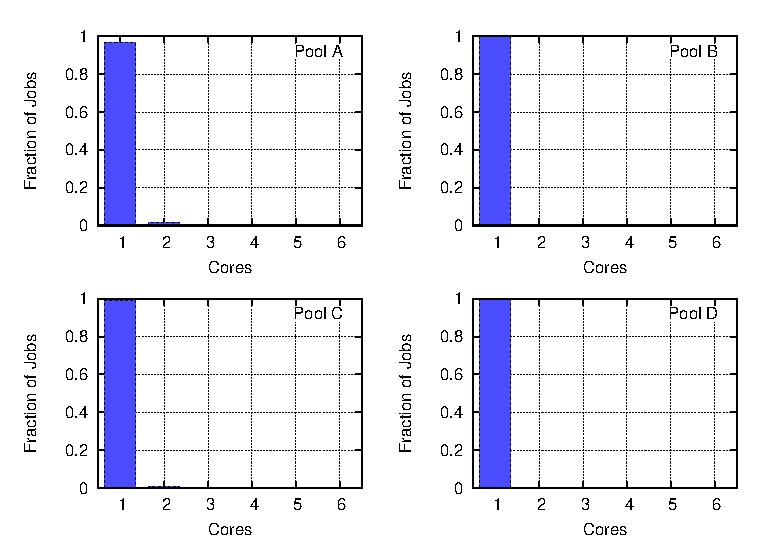
\includegraphics{figures/cores_multiplot.eps}
\caption{Jobs' cores requirements: the vast majority of the jobs are
  serial and require a single CPU core in order to execute.}
\label{fig:cores_usage_multiplot}
	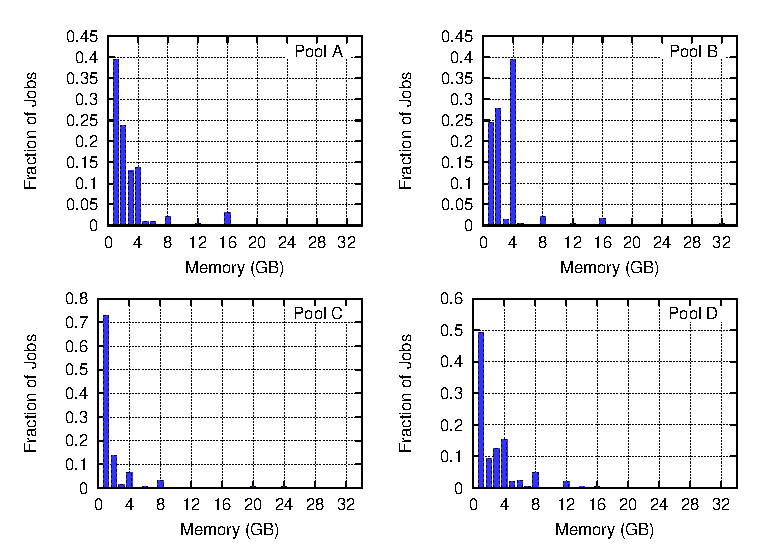
\includegraphics{figures/memory_multiplot.eps}
\caption{Jobs' memory requirements: demands are mostly 8 GB and below,
  but there are jobs that require 16 GB, 32 GB or even more memory in
  order to execute.}
\label{fig:memory_usage_multiplot}
\end{figure}

Figures \ref{fig:cores_usage_multiplot} and \ref{fig:memory_usage_multiplot}
show the distribution of the jobs' cores and memory requirements
\footnote{The requirements are specified as part of the job profile at submit time.}.
As can be seen in the figures, the vast majority of the jobs are
serial (single-thread jobs, requiring a single CPU core in order to execute).
Memory requirements are mostly 8 GB and below, but there are jobs that
require 16 GB, 32 GB, or even more memory (not shown) in order to
execute.
These observations are consistent across the pools.



\chapter{Matching Machines to Jobs}
%==================================
\label{sec:matching}

As described above, matching machines to jobs at the PPM is done by
choosing the most eligible job from the wait queue, sorting the list
of candidate machines according to some pre-defined criterion,
traversing the sorted list, and selecting the first machine on which
the job fits\footnote{This is done for practical reasons since trying
  all combinations is time consuming.}.
This is repeated again and again until either the wait queue or the
list of machines are exhausted.
At this point the PPM launches the chosen job(s) on the selected
machine(s) and waits for the next scheduling cycle.

A job may be multithreaded, but we assume that each job can fit on a
single (multicore) machine.
In principle \nb\ also supports parallel jobs (called ``MPI jobs'')
that span multiple machines, but in practice their numbers at the
present time are small.
The only added difficulty in supporting such jobs is the need to
allocate multiple machines at once instead of one at a time.

There are many criteria by which the machines can be sorted.
In this work we focus on the number of free cores and amount of free
memory, as this suits well the workload in Intel which is
characterized by compute-intensive memory-demanding jobs.
Though I/O is definitely a factor, and some jobs do perform large file
operations, there are some in-house solutions that are beyond the
scope of this work that greatly reduce the I/O burden on the
machines.

The two ways to sort the machines by available cores or memory are in
increasing or decreasing order.
Sorting them by \textit{increasing} amount of free cores or memory and
selecting the first machine on which the job fits effectively
implements the \bef\ heuristic.
\bef\ is known to result in a better packing of jobs, while
maintaining unbalanced cores (or memory) usage across the machines in
anticipation for future jobs with high resource requirements.
Sorting the machines by \textit{decreasing} amount of free cores or
memory implements the \wof\ heuristic.
\wof's advantage is in keeping resource usage balanced across
machines, which is particularly useful for mostly-homogeneous
workloads.
For completeness we also mention \fif.
\fif's advantage is in its simplicity, as it does not require the
sorting of the machines.
Our tests, however, revealed that it performs poorly in our
environment, so we do not refer to it further.

We argue that no single heuristic, when applied to a single resource in
isolation, can yield optimal performance under all workload
scenarios.
To demonstrate our point we begin by providing simple synthetic examples
showing how different heuristics match different number of jobs under
different workload conditions.
We then put theory to the test by running simulations on the
aforementioned traces, demonstrating the effectiveness of the different heuristics 
under different workloads.


\section{Synthetic Examples of Heuristics Failures}
%-----------------------------------------------------

In our examples we consider two machines, A and B, each having four
cores and 32 GB of memory.
Assume that 8 jobs are queued at the PPM in the following priority order: two jobs
of one core and 16 GB of memory, and then 6 jobs of one core and 4 GB of
memory.
As can be seen in Figure \ref{fig:wf_better_A}, \bef\ matches the first
two jobs with machine A, totally exhausting its memory, and the next
four jobs with machine B, thereby exhausting its cores.
The end result is two unutilized cores on machine A, half the memory
unutilized on machine B, and two jobs that remain pending at the PPM.
\wof\ on the other hand matches the first two jobs on different
machines, which leaves enough free space (cores and memory) for all the
remaining 6 jobs to be matched.
This is illustrated in Figure \ref{fig:wf_better_B}.

\begin{figure}\centering
\subfigure[\label{fig:wf_better_A}\bef]{
	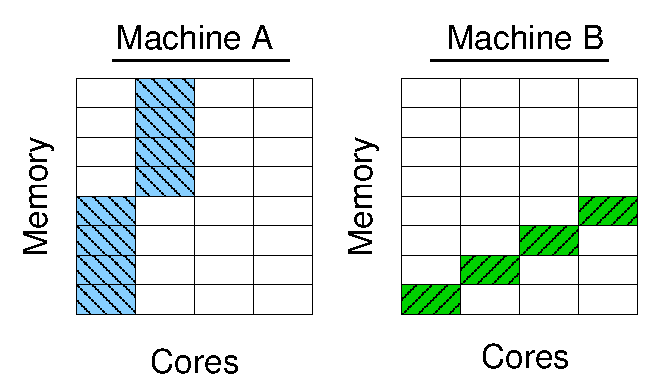
\includegraphics[width=0.45\textwidth]{figures/fig1a.eps}}
~~~~
\subfigure[\label{fig:wf_better_B}\wof]{
	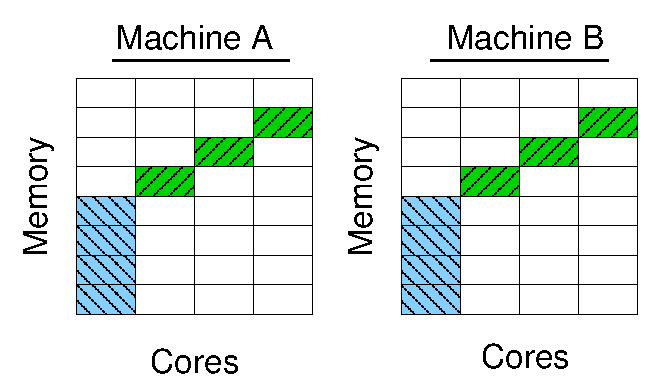
\includegraphics[width=0.45\textwidth]{figures/fig1b.eps}}
\caption{Scenario for which \wof\ (right) is better than \bef\ (left).
  Memory is depicted in 4 GB blocks.
  Shading indicates mapping of a job to a certain core and certain
  blocks of memory.
  Note that both cores and memory are mapped exclusively to distinct
  jobs.}
\label{fig:wf_better}
\end{figure}

Another example is illustrated in Figure \ref{fig:bf_better}.
The priority order here is 3 jobs of one core and 8 GB, followed by
one job of one core and 32 GB of memory.
As can be seen, \wof\ spreads the first three jobs on different
machines, which doesn't leaves enough memory for the 32 GB job to be
matched.
\bef\ on the other hand matches the first three jobs on machines A, 
which allows the 32 GB to be matched with machine B.

\begin{figure}\centering
\subfigure[\label{fig:bf_better_A}\bef]{
	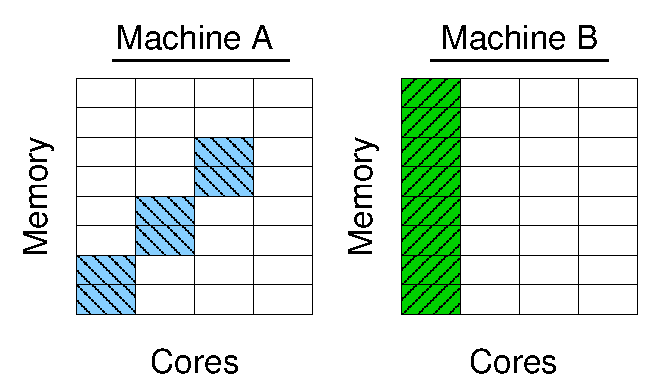
\includegraphics[width=0.45\textwidth]{figures/fig2b.eps}}
~~~~
\subfigure[\label{fig:bf_better_B}\wof]{
	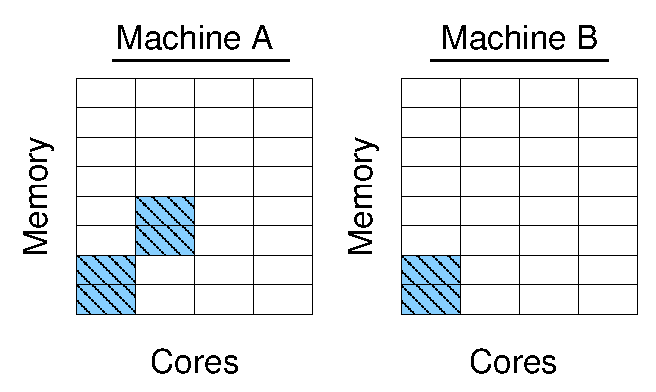
\includegraphics[width=0.45\textwidth]{figures/fig2a.eps}}
\caption{Scenario for which \bef\ (left) is better than \wof\ (right). }
\label{fig:bf_better}
\end{figure}


\section{Observations from the Workloads}
%-------------------------------------------

Machines currently available on the market typically have multi-core
CPUs and large amounts of memory.
Therefore, we may expect to see situations similar to the ones
described above.
In addition, jobs comes with core and memory requirement, and in most
cases jobs are allocated one per core.
This may waste cycles due to wait states and I/O, but makes things
much more predictable.

\begin{figure}\centering
	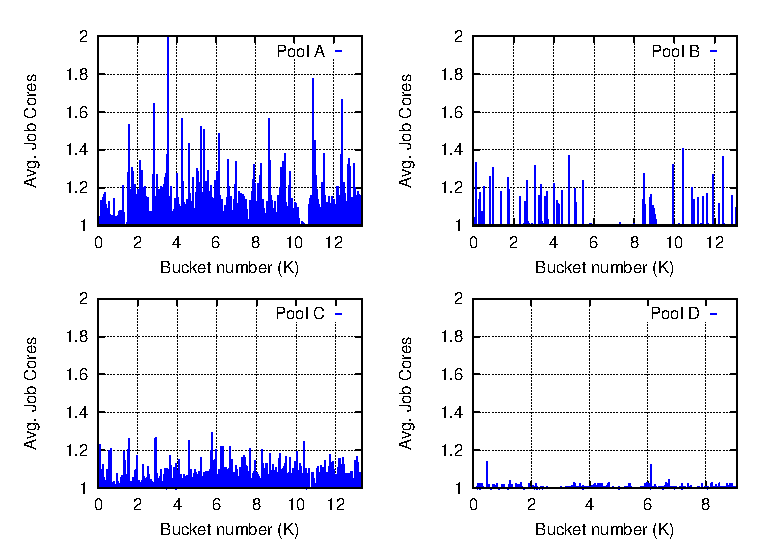
\includegraphics{figures/cores_burst.eps}
\caption{Bursts in jobs cores requirements: pool A is the burstiest.
  Pool B's bursts are sparse, while pool C's have only a small
  amplitude.
  In pool D there are virtually no bursts of jobs requiring more than
  one core.}
\label{fig:cores_burst_multiplot}
\end{figure}

To characterize the use of cores and memory in each of the pools, 
we used the traces mentioned above, 
and partitioned them into buckets of 1000 jobs each. 
This resulted in 13K buckets for pools A, B, and C, 
and 10K buckets for pool D.
Such small buckets allow us to observe bursts of activity that deviate
from the average.

\begin{figure}\centering
	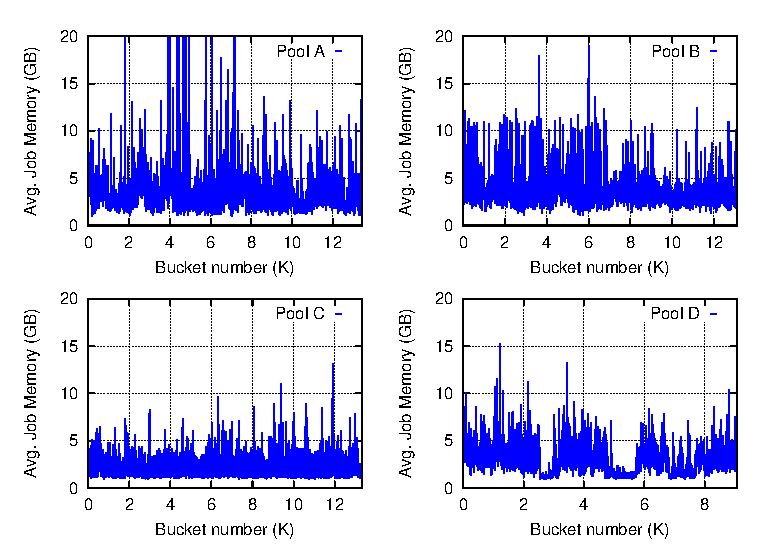
\includegraphics{figures/memory_burst.eps}
\caption{Bursts in jobs memory requirements: pools A and B are the
  most bursty; A in particular has bursts that exceed 20 GB on average.
  Pool C is somewhat steadier, while pool D exhibits periods of
  particularly low memory demands between the bursts.}
\label{fig:memory_burst_multiplot}
\end{figure}

Figures \ref{fig:cores_burst_multiplot} and
\ref{fig:memory_burst_multiplot} show the jobs' average cores and
memory requirements in each of the buckets, for each of the four pools,
respectively.
As can be seen, different pools exhibit different magnitudes of bursts
of jobs with high core or memory demands.
Pool A is the most bursty in both dimensions; it is the only pool that
had a bucket in which the average job core requirement is higher than
2, and multiple buckets in which the average memory requirement is
larger than 20 GB.

Pool B exhibits sparse bursts of jobs with high core demands, but
intense bursts of high memory requirements.
Pool C exhibits continuous moderate core demands, and also relatively
steady memory bursts.
Finally, pool D has virtually no bursts of jobs requiring more than
one core, but it does exhibit bursts of high memory demands, along
with periods of particularly low memory requirements.


\section{Comparing Heuristics}\label{sec:buckets}
%--------------------------------

To demonstrate the effectiveness of the different heuristics under different workloads 
we performed the following experiment.
We used the buckets described above, assigned all jobs in each bucket a submit
time of 0, and gave each heuristic an opportunity to try and match, in simulation, 
as many jobs as possible from each bucket on a small synthetic pool of
empty machines (total of 512 cores);
jobs that could not be matched were simply skipped.
For each bucket we then counted the number of jobs matched by each heuristic, 
and gave the winning heuristic(s) (the one(s) who matched the highest
number of jobs) a point.

%Given that each bucket contains tens of thousands of jobs, they
%cannot all be assigned to machines.

%We repeated the experiment four times: first on three homogeneous
%clusters in which all machines use the same number of cores and
%memory, and then on a heteserogeneous cluster containing a mixture of
%machines from the aforementioned clusters.

The results are shown in Figure \ref{fig:buckets}.
As can be seen, \wfc\ significantly outperforms all other heuristics 
(collecting the highest percentage of wins) in pool A. 
It is also the best heuristic in pools B, C, and D, 
but the differences there are smaller.
There is little difference among \bfm, \wfm, and \bfc, although
\wfm\ is consistently slightly better than the other two.
Notably, for pool D where there is virtually no core fragmentation 
as indicated in Figure \ref{fig:cores_burst_multiplot}
there seems to be little difference between the performance of the
different heuristics.

%This may indicate that it is best to first spread out the jobs across
%as many machines as possible.
%In fact, when all jobs are serial, \wfc\ is essentially the same as
%mapping jobs to machines in a round-robin manner.

\begin{figure}\centering                      
	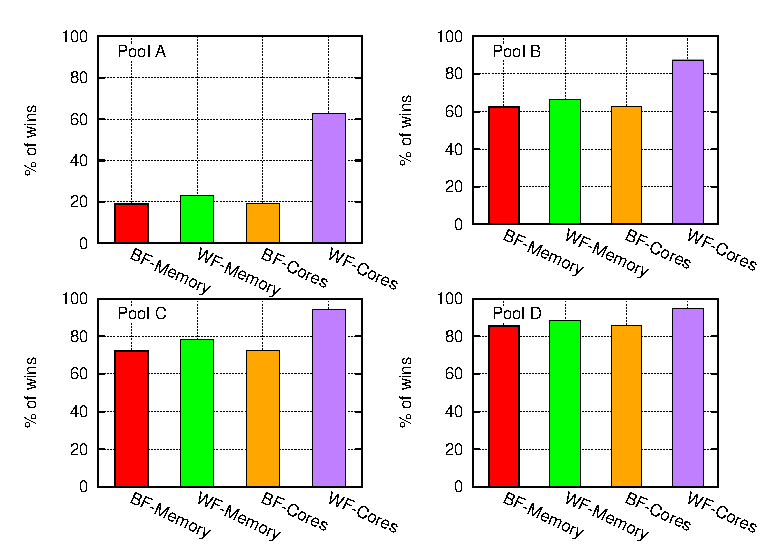
\includegraphics[width=.9\textwidth]{figures/buckets-all-no-mf.eps}
\caption{\label{fig:buckets}Percentage of wins by each heuristic:
  \wfc\ significantly outperforms the other heuristics in pool A. The
  differences in pools B, C, and D are smaller.}
\end{figure}

An important observation is that though \wfc\ appears to be the preferred heuristic, 
it did \textit{not} win in all cases. 
This is shown by the gap between the \wfc\ bars 
and the 100\% mark, indicating that in 6--37\% of the experiments
other heuristics performed better. 
These gaps are the motivation for the \mif\ heuristic
proposed next. 


\chapter{The \mif\ Heuristic}
%=============
\label{sec:mixed-fit}

As demonstrated in the previous section, none of the one-dimensional
heuristics is capable of maximizing the number of matched jobs under
all workload scenarios.
In this section we propose a new heuristic, \mif, that takes into
account both cores and memory in an attempt to overcome the problem.


\section{Balanced Resource Usage}
%-----------------------------------

The basic idea behind \mif\ is to try and reach balanced resource
utilization across both cores and memory.
This is achieved by considering the \textit{configured} ratio of cores
to memory on each machine, and matching the job with the machine on
which the ratio of \textit{used} cores to memory, together with this
job, is closest to the configured ratio.

To see how this is done, envision a grid representing possible
resource combinations (as was done in Figures \ref{fig:wf_better} and
\ref{fig:bf_better}).
Each column represents a CPU core, and each row a block of memory (the
sizes of such blocks are not really important as long as they are used
consistently; they should correspond to the smallest unit being
allocated).
Assuming that cores and memory blocks are assigned exclusively to
jobs, an allocation may be portrayed as a sequence of shaded squares
on this grid, where each job is represented by a sequence of
memory-squares in a specific core-column.

The configured ratio is represented by the diagonal of this grid, and
the used ratio by the line connecting the top-right point of the grid
with the top-right point of the last job.
\mif\ defines a parameter, $\alpha$, that denotes the angle between
these two lines.
Note that the used ratio is calculated after allocating the job being
considered, so machines on which this job does not fit are excluded
from the discussion.
\mif\ then matches the job with the machine with the minimal $\alpha$
value.
In case of a tie, the first machine with the minimal value is used.

Two important notes. First, The grid is drawn such that memory and
cores are normalized to the same scale in each machine separately, thereby
creating a square.
This prevents the scale from affecting the angle.
Second, the angle is based on lines emanating from the top right corner.
It is also possible to have a similar definition based on the origin
(i.e.\ the bottom-left corner).
Choosing the top-right corner leads to higher sensitivity when the
machine is loaded, which facilitates better precision in balancing the
resources in such cases.

Let's see an example. 
Three machines are available, each with 4 cores and 32 GB of memory.
Machine A already has one job with 24 GB, Machine B has 2 jobs
with 8 GB each, and Machine C has one job with 2 cores and 4 GB memory
and another job with 1 core and 4 GB memory.
The next job that arrives requires one core and 8 GB of memory.
The various $\alpha$ values of all three machines including the newly
arrived job are demonstrated in Figure \ref{fig:fig3}.
The machine selected by \mif\ in this case is B where
$\alpha=0$.

\begin{figure}\centering
	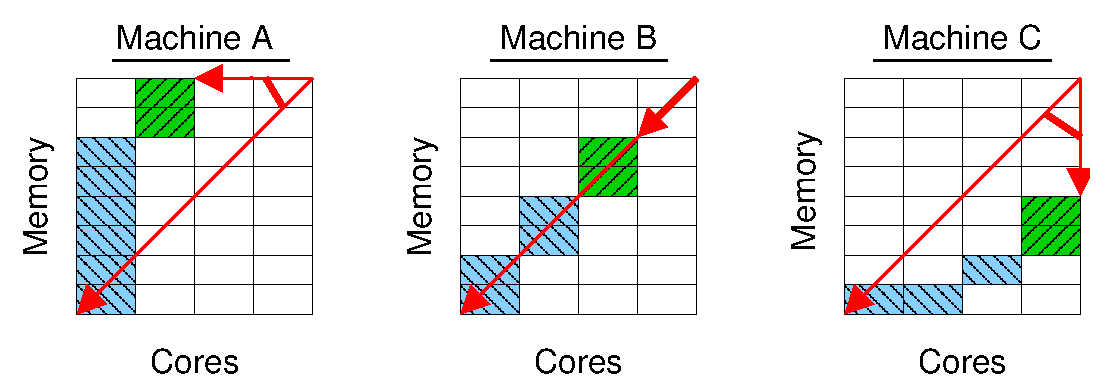
\includegraphics[width=0.75\textwidth]{figures/fig3.eps}
\caption{Example of various $\alpha$ angles calculated by \mif. The
selected machine in this case is B where $\alpha=0$.}
\label{fig:fig3}
\end{figure}

To demonstrate why this may be expected to improve over the previous
heuristics we will use the same examples we used above.
Consider Figure \ref{fig:wf_better}, where \wof\ yielded the best
match.
After matching the first 16 GB job with machine A, \mif\ will 
match the second 16 GB job with machine B, as this will lead to a
smaller $\alpha$ value as can be seen in Figure \ref{fig:fig4}.
It will then match the remaining 4 GB jobs with both machines
until all cores get utilized.
As can be seen in Figure \ref{fig:mf_final} the end result is identical
to \wof.

\begin{figure}\centering
\subfigure[\label{fig:fig4}Options for placing the 2'nd job. The angle
  on machine B is smaller.]{
	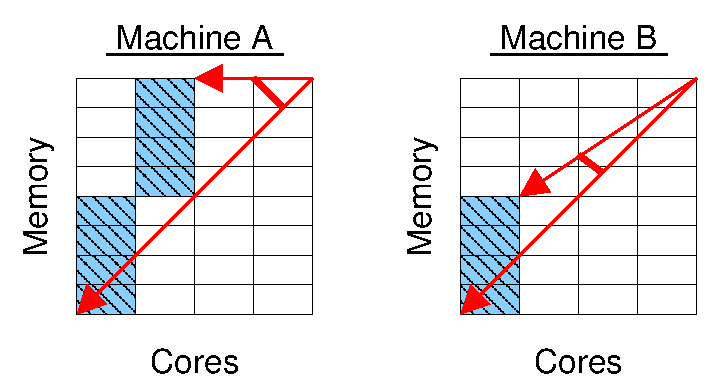
\includegraphics[width=0.45\textwidth]{figures/fig4.eps}}
~~~~
\subfigure[\label{fig:mf_final}Final allocation by \mif.]{
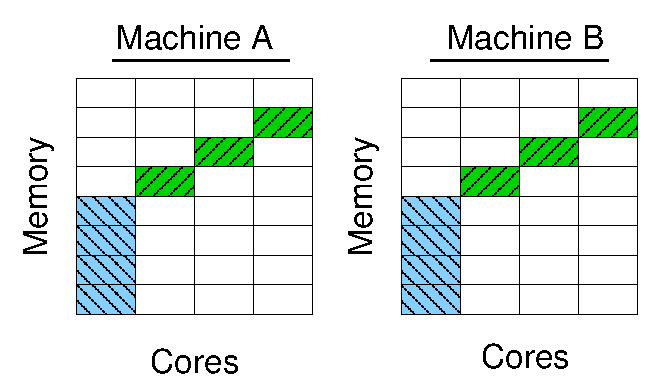
\includegraphics[width=0.45\textwidth]{figures/fig1b.eps}}
\caption{\mif\ behavior for the example in Figure \ref{fig:wf_better}.
  The end result is identical to \wof.}
\end{figure}

%\begin{figure}\centering
%	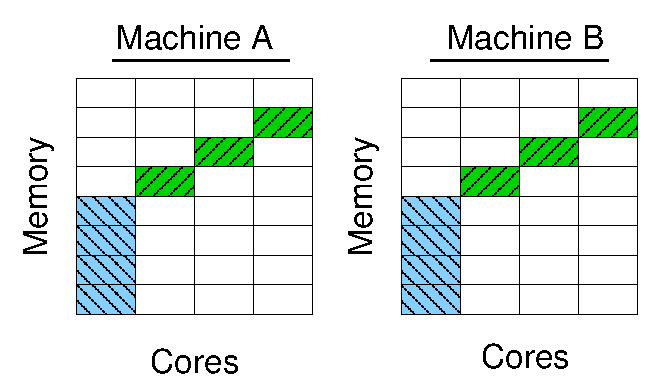
\includegraphics[width=0.45\textwidth]{figures/fig1b.eps}
%\caption{Jobs allocated by \mif\ for Example 1.}
%\label{fig:mf_final}
%\end{figure}

Next, lets re-examine Figure \ref{fig:bf_better} where \bef\ yielded the
best results.
In this scenario \mif\ will match the first three 8 GB jobs with
machine A, and then the 32 GB job with machine B, replicating the
behavior of \bef.
Note that $\alpha$ would have been the same for the second 8 GB,
whether it would have been matched on machine A or B.
But as noted above, in such cases the \fif\ heuristics is used as a
tie breaker and hence the job is matched with machine A.
As can be seen in Figure \ref{fig:mf_final2} the end result is
identical to \bef.

\begin{figure}\centering
	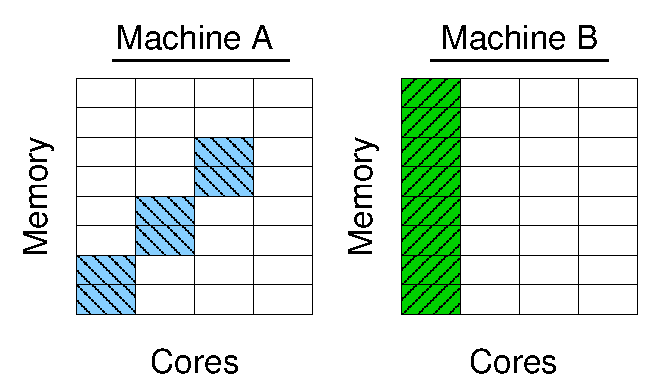
\includegraphics[width=0.45\textwidth]{figures/fig2b.eps}
\caption{Jobs allocated by \mif\ for the Example in Figure
  \ref{fig:bf_better}.
  The result is identical to \bef.}
\label{fig:mf_final2}
\end{figure}


\section{\mif's Results}
%------------------------------

To check the performance of \mif\ we repeated the buckets 
experiment from Section \ref{sec:buckets}, 
but this time including \mif\ in the set of competing heuristics.
The results are shown in Figure \ref{fig:buckets-all}.
As can be seen, \mif\ wins by only a small margin in pool A, 
performs similarly to \wfc\ in pools B and D, and is slightly outperformed by \wfc\ 
in pool C.

\begin{figure}\centering
	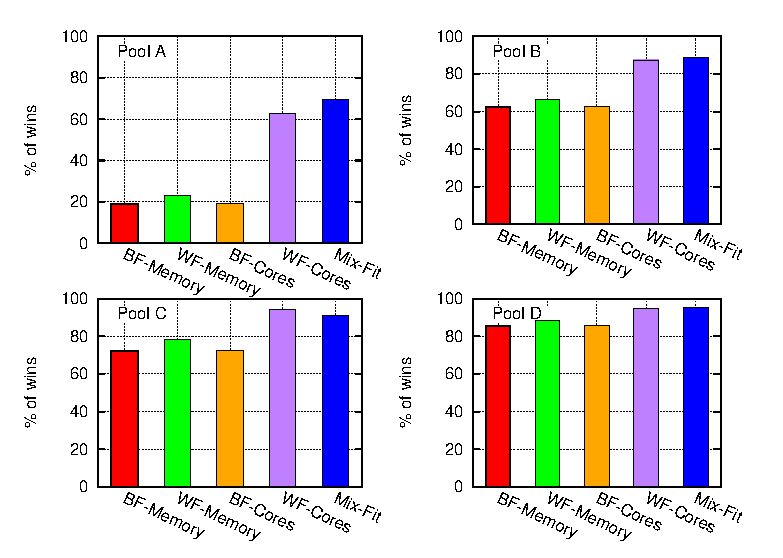
\includegraphics[width=.9\textwidth]{figures/buckets-all.eps}
\caption{Percentage of wins by each heuristic: \mif\ wins by only a
  small margin in pool A, performs similarly to \wfc\ in pools B and
  D, and is slightly outperformed by \wfc\ in pool C.}
\label{fig:buckets-all}
\end{figure}

These results are counterintuitive, since in a two-dimensional
environment of cores and memory, where both resources are subject to
sudden deflation by bursts of jobs with high demands, a reasonable
strategy would be to try and balance the usage between the resources,
in order to secure a safety margin against bursts of any kind.
This strategy, however, which \mif\ employs, seems to yield some
improvement only under the most bursty situations (pool A).
This leads us to default to a meta-heuristic, \maj, which is described
next.

%To try and quantify the magnitude of this gap, we checked how many
%jobs were scheduled in buckets that \mif\ did not have the best schedule.
%In each such bucket, we measured the delta of jobs between the best
%algorithm in that particular bucket and \mif.
%Figure \ref{fig:mf-damage} shows the results.
%The results are that
%in those cases where \mif\ is not the best, \mif\ schedules 25--48
%jobs less than the best algorithm on average, which is around 0.25\%
%of the pool capacity.
%In other words, the difference was insignificant and \mif\ was very
%close to the best result.

%\begin{figure}\centering
%	\includegraphics[width=0.45\textwidth]{figures/mf-damage.eps}
%\caption{Number of jobs the best algorithm schedules more than \mif\, in the
%cases that \mif\ was not the best.}
%\label{fig:mf-damage}
%\end{figure}


\chapter{The \maj\ Meta-Heuristic}
%=================================
\label{sec:max-jobs}

The experiment described above indicates that counterintuitively, 
\mif\ does not yield the best performance in all pools.
As an alternative, we therefore suggest the use of the \maj\ meta-heuristic.

%[Dror - lets leave that (how real systems work) to when we describe the load results, which are also different from the buckets].
%While the experiments done above indicate that \mif\ should provide
%good performance, they are conducted in a highly artificial setting:
%a large number of jobs is scheduled at once on a previously empty
%pool.
%But real systems work in an on-line setting, suffering from
%fragmentation and lack of information regarding future events.
%As results described below show, in such realistic situations
%\mif\ does not always provide the best performance.
%We therefore suggest the use of the \maj\ meta-heuristic.

A meta-heuristic is an algorithm that employs other heuristics as
subroutines.
In our case, \maj\ uses all of the heuristics described before: \bfc,
\bfm, \wfc, \wfm, and \mif.
At each scheduling cycle, \maj\ picks the best schedule produced by
any of these heuristics for this cycle.
In other words, the meta-algorithm runs all the available heuristics
as black-boxes and selects the one with the best result for the
currently queued jobs.
The target function defining ``best'' is maximizing the
number of jobs assigned to machines in this cycle.
Importantly, additional heuristics can be added later and the system
will take advantage of them in those cases that they perform the best.

Pseudo-code for the \maj\ meta-heuristic is given in Figure
\ref{fig:max-jobs}.

\begin{figure}\centering
\fbox{\parbox{7cm}{
    \begin{tabbing}
    xx\=xxxxx\=xxxxx\=\+\kill
    L -- list of heuristics\\
    S -- list of proposed schedules (mapping jobs to hosts)\\[3mm]

    foreach heuristic H in L\\
    \> S[H] = H.Schedule(waitingQueue)\\
    maxJobsSchedule = MaxJobsSchedule(S)\\
    Dispatch(maxJobsSchedule)
    \end{tabbing}
}~~}
  \caption{The \maj\ meta-heuristic.}
  \label{fig:max-jobs}
\end{figure}


\chapter{Simulation Results}
%===========================
\label{sec:sim_results}

To experiment with \maj, \mif\ and the rest of the heuristics, we
developed a Java-based event-driven simulator \cite{simba} that mimics the
matching behavior at the PPM.
The simulator accepts as input a jobs trace file, 
a machines configuration file, and a parameter defining which matching heuristic
to apply.
It first loads the two files into memory, building an event queue of
job arrival events sorted according to the timestamps from the trace 
(hence preserving the original arrival order and inter-arrival times of the jobs), 
and a list of machine objects according to the configuration.

The scheduling function is invoked by the scheduler at regular
intervals, as is commonly done in many large-scale systems.
In our simulations we used an interval of 30 seconds.
This allows the scheduling overhead to be amortized over multiple jobs
that are handled at once, 
and may also facilitate better assignments of jobs to machines, because
the scheduler can optimize across a large number of jobs rather than
treating them individually.

In each scheduling cycle, the scheduler begins by picking the first
arrival event from the queue and trying to match a machine to the
arriving job using the selected heuristic\footnote{For simplicity we skipped the fair-share calculation.}.
If the matching succeeds the job is marked as ``running'' on the
selected machine, and a completion event is scheduled in the event
queue at a timestamp corresponding to the current time plus the job's
duration from the trace.
Otherwise a reservation is made for the job.
Specifically the machine with the highest available memory is reserved
for the job for its future execution, thus preventing other jobs from
being scheduled to that machine during the rest of the scheduling cycle. 

%During scheduling in simulator, jobs where sorted by their arrival order. We
%selected that startegy rather than mimic that actual fairshare allocation that
%happened at PPM for simplicity. The fairshare calculation was out of the scope
%for our paper.

For the workload we used the traces that were described in Section
\ref{sec:matching}, and which contains 9--13 million jobs each.
The parameters we used from the traces are the jobs' arrival times,
runtime duration, and the number of cores and amount of memory each
job requires in order to execute (see Figures
\ref{fig:cores_usage_multiplot} and \ref{fig:memory_usage_multiplot}
for the distributions).
For the machines we used a special \nb\ command to query the present
machine configurations from each of the pools on which the traces were
collected.

Our initial simulations revealed that
the original load in the traces is too low for the wait queue in the
simulated PPM to accumulate a meaningful number of jobs.
This may stem from fact that the load in the month in which the traces
were collected was particularly low, or that the configuration
has changed by the time we ran the machines query (a few months later). 
%fact that we included machines that were actually not usable.
In any case the results were that all heuristics performed the same. 

To overcome this problem we increased the load by multiplying the jobs
arrival time by a factor, $\beta$, that is less than or equal to one.
The smaller the value of $\beta$, the smaller the inter-arrival times
become between the jobs, which increases the rate of incoming jobs and
the load on the simulated pool. 
We ran high-load simulations with $\beta$ 
values ranging between 0.58--0.95. In the figures below, we translate the
$\beta$ values into an actual load percentage for each pool.

Metrics that were measured are the average wait time of jobs, the
average slowdown, and the average length of the waiting queue during the
simulation.
The results are shown in Figures \ref{fig:avg-wait-with-max-jobs} to
\ref{fig:avg-waitqueue-with-max-jobs}, for each metric, respectively.
Since the metrics are dependent and the results are similar between the metrics, 
we will only discuss the differences between the heuristics and pools.

%\begin{figure}\centering
%	\includegraphics[width=0.9\textwidth]{figures/avg-wait.eps}
%\caption{Average wait time of jobs.}
%\label{fig:avg-wait}
%\end{figure}

%\begin{figure}\centering
%	\includegraphics[width=0.9\textwidth]{figures/avg-slowdown.eps}
%\caption{Average slowdown of jobs.}
%\label{fig:avg-slowdown}
%\end{figure}

%\begin{figure}\centering
%	\includegraphics[width=0.9\textwidth]{figures/avg-waitqueue.eps}
%\caption{Average wait-queue length.}
%\label{fig:avg-waitqueue}
%\end{figure}

\begin{figure}\centering
	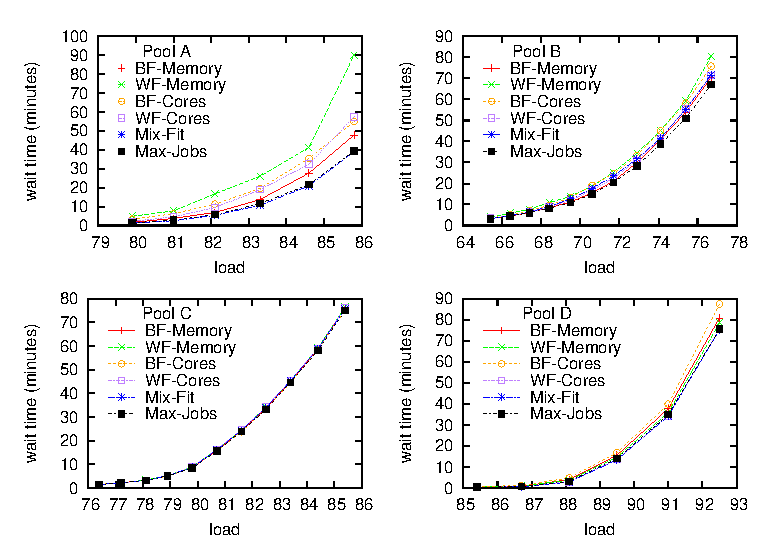
\includegraphics[width=1.0\textwidth]{figures/avg-wait-with-max-jobs.eps}
\caption{Average wait time of jobs.
System load is expressed as percent of capacity.}
\label{fig:avg-wait-with-max-jobs}
\end{figure}

\begin{figure}\centering
	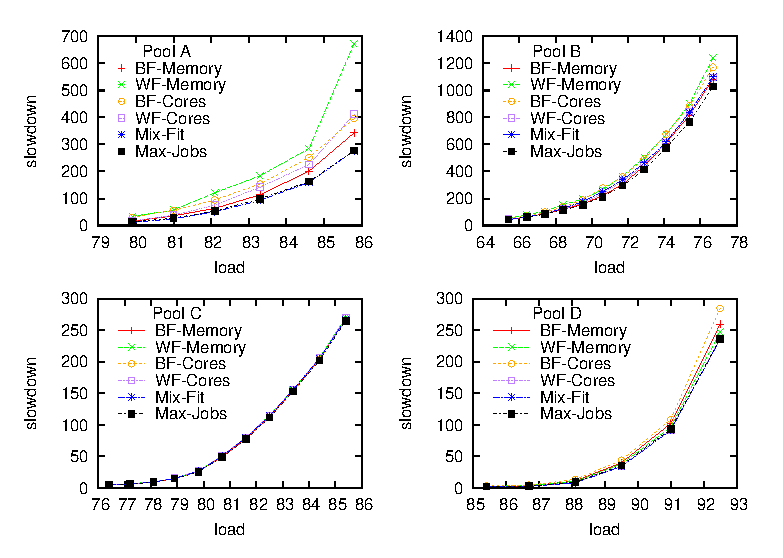
\includegraphics[width=1.0\textwidth]{figures/avg-slowdown-with-max-jobs.eps}
\caption{Average slowdown of jobs.}
\label{fig:avg-slowdown-with-max-jobs}
\end{figure}

\begin{figure}\centering
	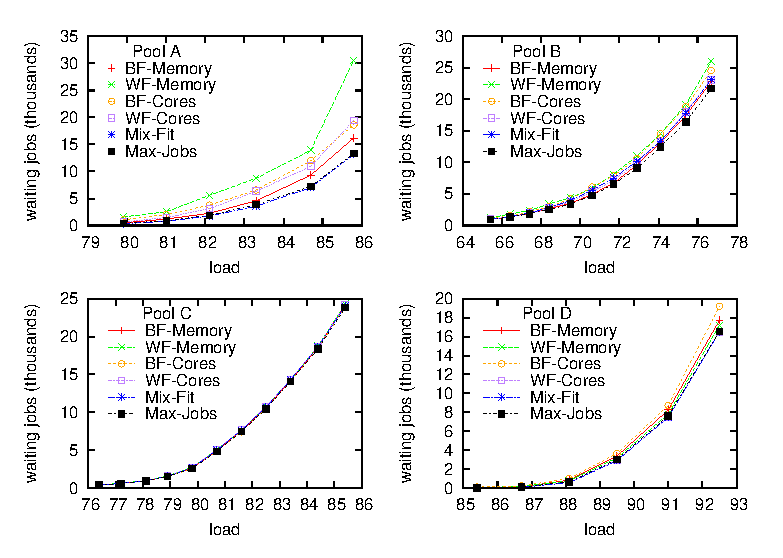
\includegraphics[width=1.0\textwidth]{figures/avg-waitqueue-with-max-jobs.eps}
\caption{Average wait-queue length.}
\label{fig:avg-waitqueue-with-max-jobs}
\end{figure}

In correlation with the buckets experiment in Figure \ref{fig:buckets-all}, 
\mif\ showed marked improvement over the other heuristics in pool A, 
and was able to reduce the waiting time by 22\%, slowdown by 23\%, and queue
length by 22\% under the highest loads simulated.


The second-best heuristic on pool A, \bfm, appears to slightly outperform \mif\ 
in pool B, especially in the mid-range load, as opposed to the buckets
experiment.
This may be caused by the fact that pool B had the most intense bursts
of high memory demands and the largest fraction of 4 GB jobs, making
the conservation of memory resources of prime importance.
At the same time, \bfm\ performs relatively poorly on pool D.

Similarly, \wfc\ that was the best heuristic in the buckets experiment
(except for \mif) appears to perform poorly in the load simulation in
both pools A and B.
This may stem from the fact that the buckets experiments were 
conducted in a highly artificial setting where all jobs were presented
in advance, and were matched to empty clusters of machines.
In such a scenario \wfc\ --- which is similar to round-robin
allocation --- performed well, but when confronted with a continuous
on-line scenario, where machines typically already have some of their
resources taken, it did not.
This is another indication that challenges faced by on-line schedulers are
different from those faced by batch (or off-line) schedulers, and that
it is important to match the simulation type to the system type.
In our case this means that the dynamic simulations described here are
more relevant than the bucket experiments used above.

In pool C all the heuristics achieved essentially the same performance.
This reflects an unchallenging workload that can be handled by any heuristic.

Finally, in pool D \mif\ had similar results to the second best heuristic, \wfc.
It looks like the non-bursty nature of that pool gives an advantage to balancing
heuristics such as \wfc. 

%We therefor do not discuss pool D any more.
%of high memory usage jobs.
%\wfc\ was one of the worst heuristics, in contrast with its good
%performance in the bucket experiments described before.
%This indicates that the challenges faced by on-line schedulers are
%different from those faced by batch (or off-line) schedulers, and that
%it is important to match the simulation type to the system type.
%In our case this means that the dynamic simulations described here are
%more relevant than the bucket simulations used above.

Figure \ref{fig:max-jobs-selected} shows the fraction of
times each heuristic was selected by \maj.
As can be seen, \mif\ is dominant, even more than in the
above buckets experiment, but still getting as low as 73\%
in pool A.
\bfm\ is markedly better than \wfc\ especially in pools A and D.

\begin{figure}\centering
	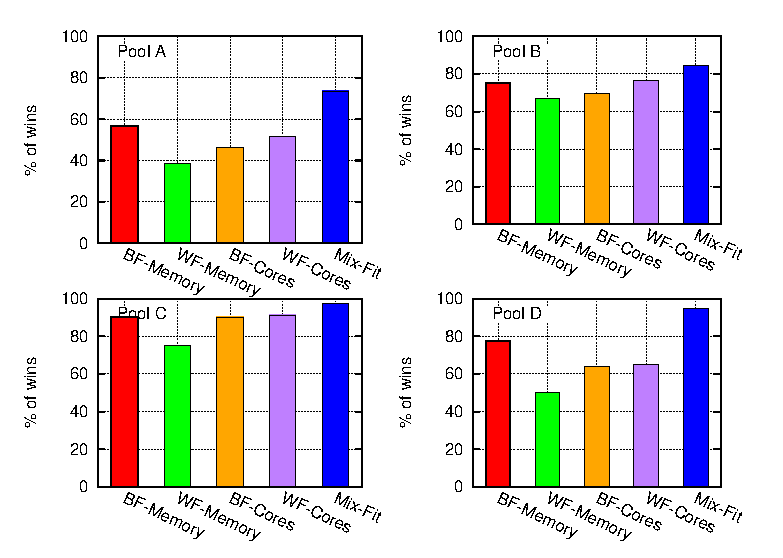
\includegraphics[width=0.9\textwidth]{figures/max-jobs-selected.eps}
\caption{Selected heuristics by \maj.
Sum is more than 100\% because in many cases several heuristics
produced the same result.}
\label{fig:max-jobs-selected}
\end{figure}

%Generally, \mif\ performed well in Pool A where bursts of cores and memory
%requirements were noticable. In other pools, \mif\ was similar or event worse
%compared to the best hueristic. 

As expected, the \maj\ meta-heuristic is the
best scheme all around, and seems to be largely robust against workload and configuration variations.
This is due to the fact that it uses the best heuristic at each
scheduling cycle.
However, its final result (in terms of average performance across all
the jobs in the trace) is not necessarily identical to that of the
best heuristic that it employs.
On one hand, \maj\ can be better than each individual heuristic, as
happens for example in pool B.
This is probably because it can mix them as needed, and use a
different heuristic for different situations as they occur.
On the other hand, \maj\ is sometimes slightly inferior to the best
individual heuristic, as seen for example in pool A.
This is probably due to situations in which packing jobs very densely
leads to reduced performance in a successive scheduling round.


\chapter{Related Work}
%=====================
\label{sec:related}

There are very few externally available publications that relate to \nb.
Zhang et al.\ investigated the use of dynamic rescheduling of
\nb\ jobs between pools which improves utilization at the farm level
\cite{Zhang2010}.
Our work in effect complements theirs by focusing on utilization
improvements within the individual pools.

The question of assigning machines to jobs has received some attention
in the literature.
Xiao et al.\ studied a problem similar to ours and also concluded that
one-dimensional strategies yields sub-optimal performance
\cite{Xiao02dynamiccluster}.
In their work, however, cores are considered shared resources, and
thus the investigation focused on the interference between the jobs.
Amir et al.\ proposed a load balancing scheme where the targets for
process migration are selected so as to avoid saturation of any single
resource \cite{amir00}.
This is similar to avoiding high $\alpha$ values in our terminology.

The idea of symbiotic scheduling is also related to our work.
Symbiotic scheduling attempts to find sets of jobs that complement
each other and together use the system resources effectively.
This was initiated in the context of hyperthreading (or simultaneous
multithreading) processors \cite{snavely00,eyerman10},
and extended also to the domain of clusters \cite{weinberg06}.

Meta-schedulers like the \maj\ approach have also been used before.
For example, Talby used such a meta-scheduler to select among different
versions of backfilling in scheduling large-scale parallel machines
\cite{talby05}.
However, this was done by simulating recent work in the background and
then switching to the version that looks best.
Such an approach depends on an assumption of locality, meaning that
the future workload will also benefit from this version.
In our work we actually run all the contending variants on the jobs in
the queue, and select the one that indeed achieves more assignments.

Another meta-scheduler example is the portfolio scheduler
\cite{Deng1305Protfolio} that was developed in parallel to our work. The
portfolio scheduler is a general-purpose mechanism that applies
to scientific computing with various target functions for scheduling. \maj\ on
the contrary, applies to batch systems and its target function is specified as
maximizing the total number of running jobs.

It should be noted that due to the assumption that cores and memory
are allocated exclusively to jobs, our problem is not directly related
to the well-known 2D bin-packing problem.
In particular, it is not allowed to pack multiple jobs with limited
memory requirements onto the same core \cite{mishra11}. 
It does, however, correspond the problem of allocating virtual machines
to physical servers which has gained much attention in resent years.
This has been called the \emph{vector bin-packing problem}, since the
allocation can be depicted as the vector-sum of vectors representing
the resource requirements of individual virtual machines \cite{panigrahy11}.
This directly corresponds to our depiction of rectangles that connect
at their corners in Figures \ref{fig:wf_better}, \ref{fig:bf_better}, etc.

The ideas suggested for vector bin-packing are all very similar to our
\mif\ algorithm.
For example, they are also based on normalizing the resources and
creating a square (or multi-dimensional cube, if there are more
resources than 2).
The available resources are then represented by a diagonal vector, the
consumption by other vectors, and the basic idea is to try to make
these vectors close to each other.
However, the details may differ.

Mishra and Sahoo \cite{mishra11} describe the SandPiper algorithms
used in Xen, and the VectorDot algorithm \cite{singh08}.
They show that both suffer from failures similar to the ones we
demonstrated in Section \ref{sec:matching}.
For example, the VectorDot algorithm uses the dot product of the
consumed resources vector and the request vector to identify requests
that are orthogonal to the current usage, and thus may be expected to
complement it.
However, this is subject to artifacts because the lengths of the
vectors also affect the result.
They then suggest a rather complex approach for identifying
complementary vectors based on a discretization of the space called
the ``planar resource hexagon''.
They did not, however, evaluate its performance compared to existing
heuristics.

Panigrahy et al.\ study a wide range of \fif-Decreasing-based
algorithms \cite{panigrahy11}.
The idea is to combine the requirements for different resources in
some way into a single number, and then pack in a decreasing order.
However, this approach loses the important geometrical structure of
the problem.
They therefore also consider heuristics based on the dot product or
the maximal required resource.
The evaluations are based on presumed synthetic distributions.

Compared with these previous works, our approach of using just the
angle between two vectors is among the simplest.
Basing the comparison at the top-right corner for improved
discrimination seems to be novel.
It would be interesting to evaluate the effect of these details, but
our results so far indicate that they may not have much impact for
real workloads.

Lee et al.\ investigated the problem of virtual machines allocation
taking into consideration the consolidation of virtual machines onto
the same physical platform, and the possible resulting resource
contention \cite{sangmin}.
In principle such considerations are also applicable to our work.
However, we note that the configuration of \nb\ pools is such that I/O
and bandwidth are seldom a bottleneck.

Finally, it is important to remember that since the PPM considers 
the jobs one at a time
there is a limit on the optimizations that can be applied. 
Looking further into the queue and considering more than one job 
may yield significant improvements \cite{Shmueli05backfillingwith}.


\chapter{Conclusions}
%====================
\label{sec:conclusions}

Matching jobs with resources is an NP-hard problem.
The common practice is therefore to rely on heuristics to do the
matching.
In this work we investigated the problem of resource matching in
Intel's compute farm, and showed that none of the well-known
heuristics such as \bef\ or \wof\ yield optimal performance in
all workload scenarios and cases.
This stems from two reasons.
First, these heuristics focus on a single resource, either cores or
memory, whereas in reality the contention may apply to the other
resource.
To address this problem we implemented a specialized heuristic, \mif,
that takes both resources into account and tries to create an
assignment that leads to a balanced use of the resources.
In principle this can be extended to more than two resources.
While this too failed to be optimal in all cases, it did show some
improvement under certain conditions.

Second, the nature of dynamically changing demands prevent a specific
use-case-tailored algorithm to be optimal for all cases.
For that, we proposed a meta-heuristic called \maj, that is not
tailored to a specific workload or scenario.
Rather, it uses the other heuristics as black-boxes, and chooses, in
every scheduling cycle, the one that yields the maximal number of
matched jobs.
We have demonstrated through simulations that max-jobs is highly
competitive with all the individual heuristics, and as such is robust
against changes in workload or configuration.

%In the future we plan to continue our investigation in several
%directions.
%One is a more detailed investigation of the impact of using
%Heterogeneous machines, in which the ratio of cores to memory is not
%fixed.
%Another is to consider how to relieve the constraint that cores are
%allocated exclusively to distinct jobs, without any time slicing.




\end{spacing}

%end of main section


\bibliographystyle{plainnat}
\bibliography{references}

\newpage{}

\begin{comment}
It is possible to create the Hebrew part in \LyX{}, but this is less
of our concern. Any typesetting software like \LyX{} (or Word or OpenOffice)
is as good for this purpose. After creating the PDF file from the
Hebrew document, include it here using the Insert -> File -> External
material -> PDFpages (one of the options). See the example below. 
\end{comment}


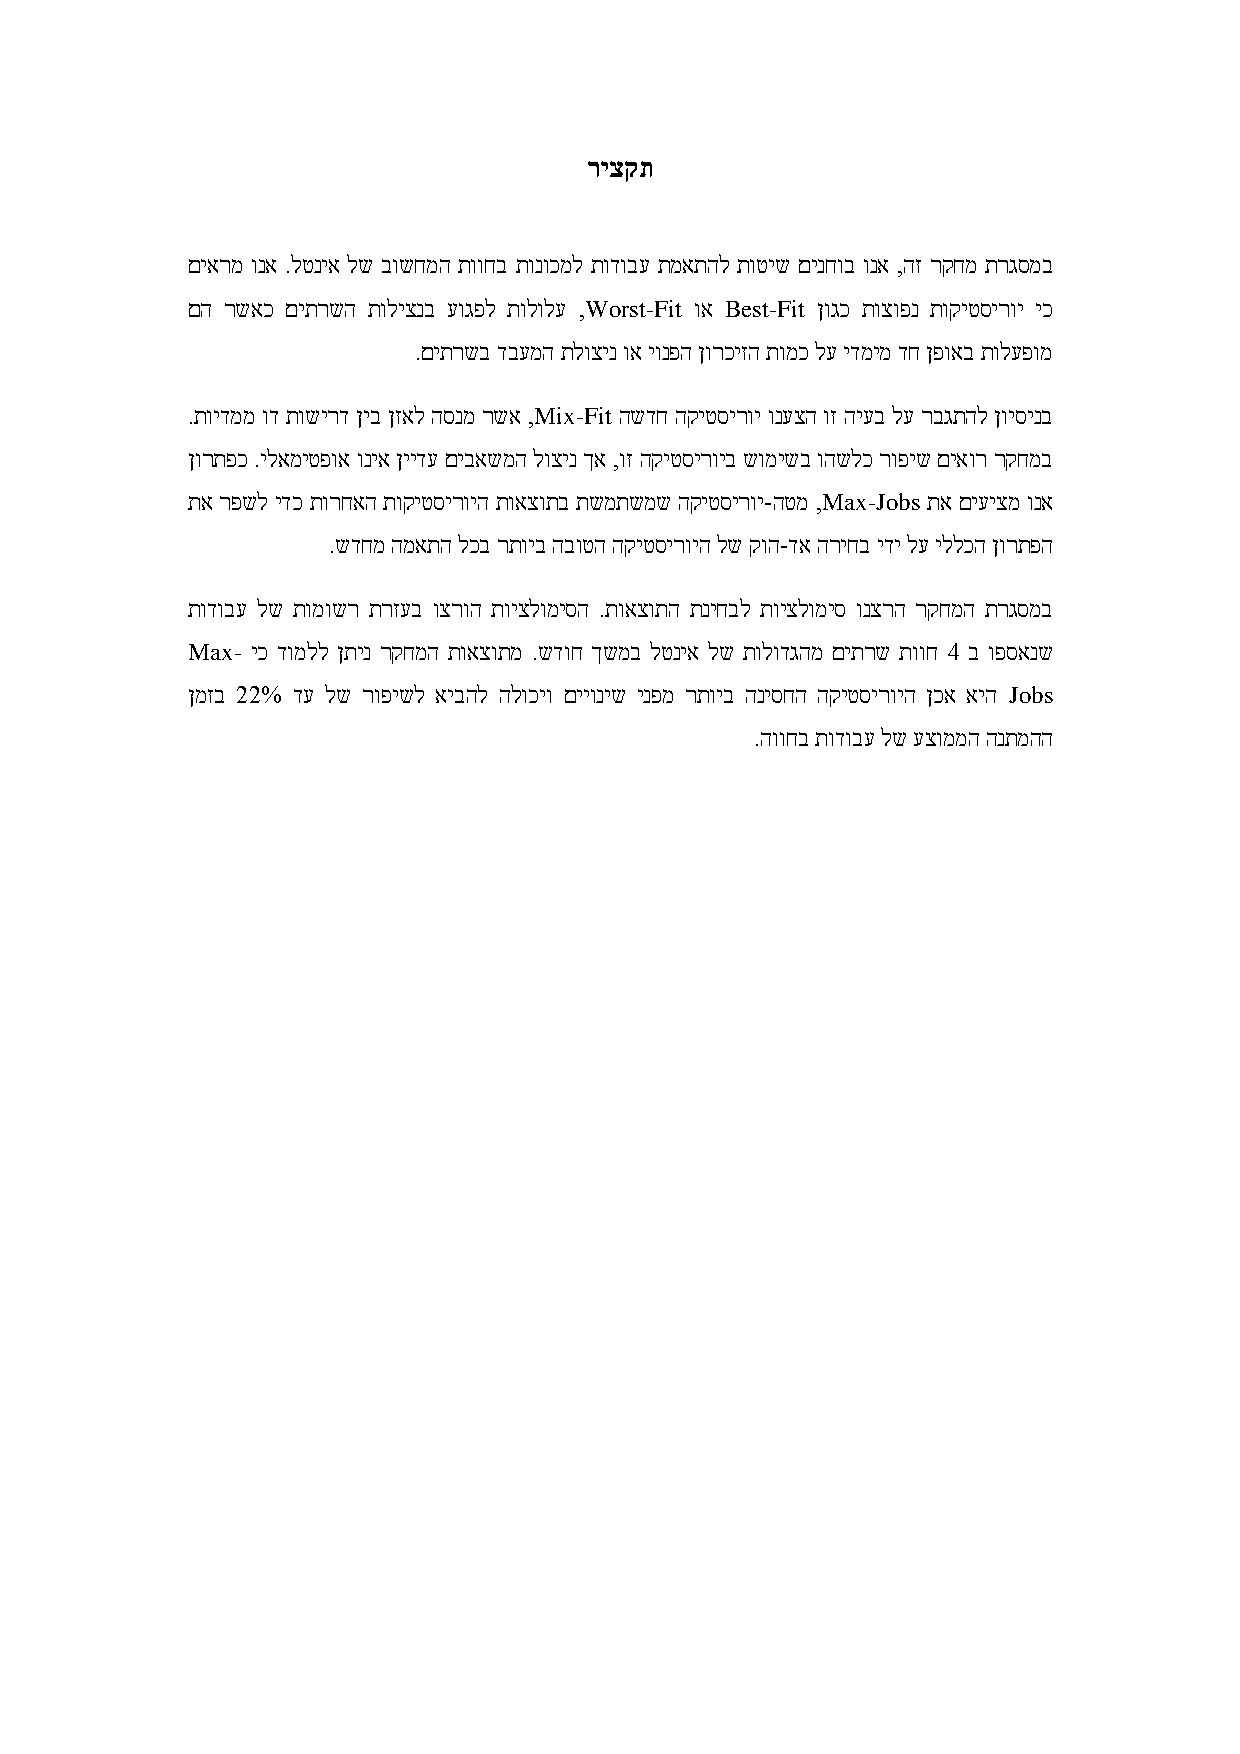
\includepdf[pages=-]{hebrew_part}
\end{document}
